% !TeX root = ../main.tex


\begin{frame}
  \frametitle{{\small Coverage Testing for Topological  {\color{red} Scalar Field} Analysis}}

  \begin{textblock*}{12cm}(1cm,2cm)
    A real-valued function $f : D \to \R$.
  \end{textblock*}

  \begin{textblock*}{12cm}(1cm,5.3cm)
    
\includegraphics[trim=200 200 200 200, clip, width=0.5\textwidth]{figures/surf/side_all.png}
    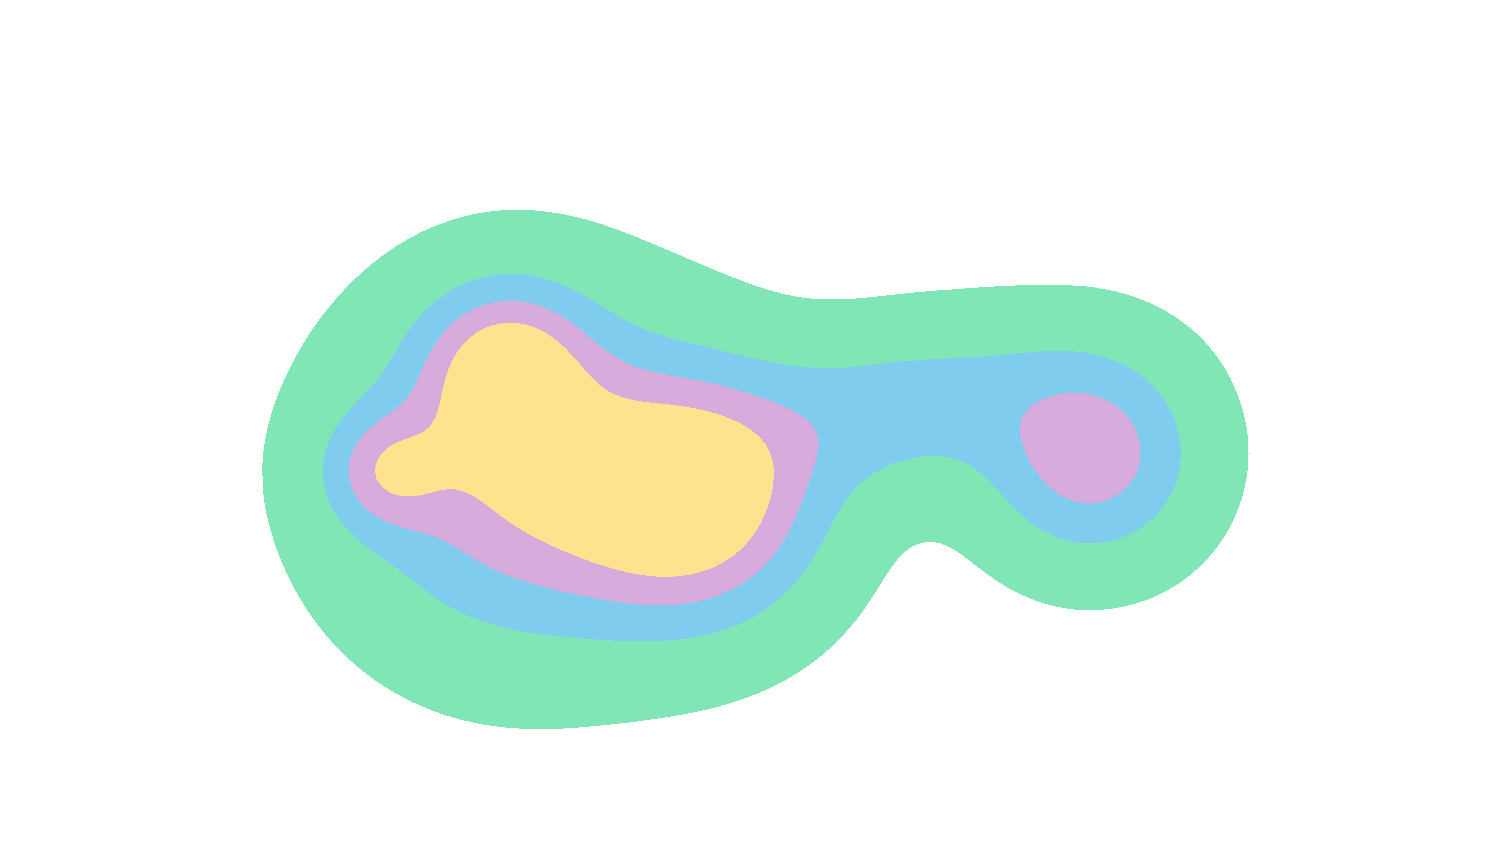
\includegraphics[trim=250 0 50 100, clip, width=0.4\textwidth]{figures/surf/top_all.png}
  \end{textblock*}
\end{frame}

\begin{frame}
  \frametitle{{\small Coverage Testing for {\color{red} Topological Scalar Field Analysis}}}
  % How the \emph{shape} of $f^{-1}((-\infty,\alpha])$ changes with $\alpha\in\R$.
  \begin{textblock*}{12cm}(1cm,2cm)
    How the \emph{shape} of $f$ changes with $\alpha\in\R$.\vspace{1ex}%   \only<2>{$\alpha=0.2$}\only<3>{$\alpha=0.5$}\only<4>{$\alpha=0.8$}\only<5>{$\alpha=1$}

    \only<2-5>{Known as \emph{persistent homology}.}
  \end{textblock*}

  \begin{textblock*}{12cm}(1cm,3.5cm)
    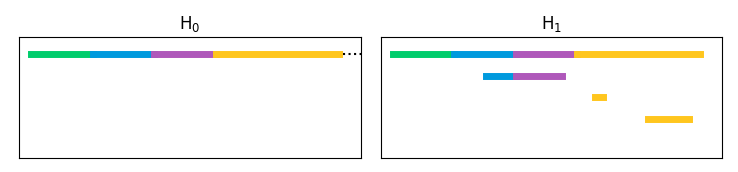
\includegraphics[width=0.6\textwidth]{figures/scalar_barcode_true.png}
  \end{textblock*}

  \begin{textblock*}{12cm}(1cm,5.3cm)
    \includegraphics<1>[trim=200 200 200 200, clip, width=0.5\textwidth]{figures/surf/side_all.png}
    \includegraphics<1>[trim=250 0 50 100, clip, width=0.4\textwidth]{figures/surf/top_all.png}
    \includegraphics<2>[trim=200 200 200 200, clip, width=0.5\textwidth]{figures/surf/side_B.png}
    \includegraphics<2>[trim=250 0 50 100, clip, width=0.4\textwidth]{figures/surf/top_B.png}
    \includegraphics<3>[trim=200 200 200 200, clip, width=0.5\textwidth]{figures/surf/side_C.png}
    \includegraphics<3>[trim=250 0 50 100, clip, width=0.4\textwidth]{figures/surf/top_C.png}
    \includegraphics<4>[trim=200 200 200 200, clip, width=0.5\textwidth]{figures/surf/side_D.png}
    \includegraphics<4>[trim=250 0 50 100, clip, width=0.4\textwidth]{figures/surf/top_D.png}
    \includegraphics<5>[trim=200 200 200 200, clip, width=0.5\textwidth]{figures/surf/side_all.png}
    \includegraphics<5>[trim=250 0 50 100, clip, width=0.4\textwidth]{figures/surf/top_all.png}
  \end{textblock*}
\end{frame}

\begin{frame}
  \frametitle{{\small Coverage Testing for {\color{red} Topological Scalar Field Analysis}}}

  \begin{textblock*}{12cm}(1cm,2cm)
    Sample $P\subset D$ of $f : D\to \R$.\vspace{1ex}


    \only<2,3>{Analyze with discrete representation.\vspace{1ex}}

    \only<3>{Cover $P^\delta = \bigcup_{p\in P}\ball^\delta(p)$.}
  \end{textblock*}

  \begin{textblock*}{12cm}(1cm,5cm)
    \includegraphics<1>[trim=200 600 200 800, clip, width=0.5\textwidth]{figures/partial3/samples}
    \includegraphics<2>[trim=200 600 200 800, clip, width=0.5\textwidth]{figures/partial3/complex}
    \includegraphics<3>[trim=200 600 200 800, clip, width=0.5\textwidth]{figures/partial3/cover}
    % \includegraphics<3>[trim=200 600 200 800, clip, width=0.5\textwidth]{figures/samples/complex1}
  \end{textblock*}
\end{frame}

\begin{frame}
  \frametitle{{\small The Topological Coverage Criterion (TCC)}}

  \begin{textblock*}{12cm}(1cm,2cm)
    \begin{small}
      Bounded domain $D$ with boundary $B$.\vspace{1ex}

      \only<2-4>{Geometric sample of $D$.\vspace{1ex}}

      \only<3,4>{Use homology to identify holes in coverage.}
    \end{small}
  \end{textblock*}

  \begin{textblock*}{12cm}(1cm,5cm)
    \includegraphics<1>[trim=200 600 200 800, clip, width=0.5\textwidth]{figures/nocover/surf}
    \includegraphics<2>[trim=200 600 200 800, clip, width=0.5\textwidth]{figures/nocover/samples}
    % \includegraphics<2>[trim=200 600 200 800, clip, width=0.5\textwidth]{figures/nocover/cover}
    \includegraphics<3>[trim=200 600 200 800, clip, width=0.5\textwidth]{figures/nocover/complex}
    \includegraphics<4>[trim=200 600 200 800, clip, width=0.5\textwidth]{figures/cover/complex}
  \end{textblock*}
\end{frame}

\begin{frame}
  \frametitle{{\small TCC $\to$ SFA}}

  \begin{textblock*}{12cm}(1cm,2cm)
    \only<1,2>{Consider partial coverage.\vspace{1ex}}

    \only<2>{Suppose points sample $f : D\to \R$.}
    \only<3>{Define our boundary as a sublevel set $B_\omega$ of $f$.}
    \only<4>{Determine coverage of $D\setminus B_\omega$.}
  \end{textblock*}

  \begin{textblock*}{12cm}(1cm,5cm)
    \includegraphics<1>[trim=200 600 200 800, clip, width=0.5\textwidth]{figures/partial/complex}
    \includegraphics<2>[trim=200 600 200 800, clip, width=0.5\textwidth]{figures/partial1/samples}
    \includegraphics<3>[trim=200 600 200 800, clip, width=0.5\textwidth]{figures/partial2/samples}
    \includegraphics<4>[trim=200 600 200 800, clip, width=0.5\textwidth]{figures/partial2/complex}
    % \includegraphics<3>[trim=200 600 200 800, clip, width=0.5\textwidth]{figures/nocover/cover}
    % \includegraphics<4>[trim=200 600 200 800, clip, width=0.5\textwidth]{figures/nocover/complex}
    % \includegraphics<5>[trim=200 600 200 800, clip, width=0.5\textwidth]{figures/cover/complex}
  \end{textblock*}
\end{frame}

\begin{frame}
  \frametitle{{\small {\color{red} \textbf{Goal:}} Analyze $f$ where we have confirmed coverage.}}

  \begin{textblock*}{12cm}(1cm,2cm)
    \begin{enumerate}
      \item<2,3> Check for coverage of $D\setminus B_\omega$,
      \item<3> Analyze $f$ in $D\setminus B_\omega$.
    \end{enumerate}
  \end{textblock*}

  \begin{textblock*}{12cm}(1cm,5cm)
    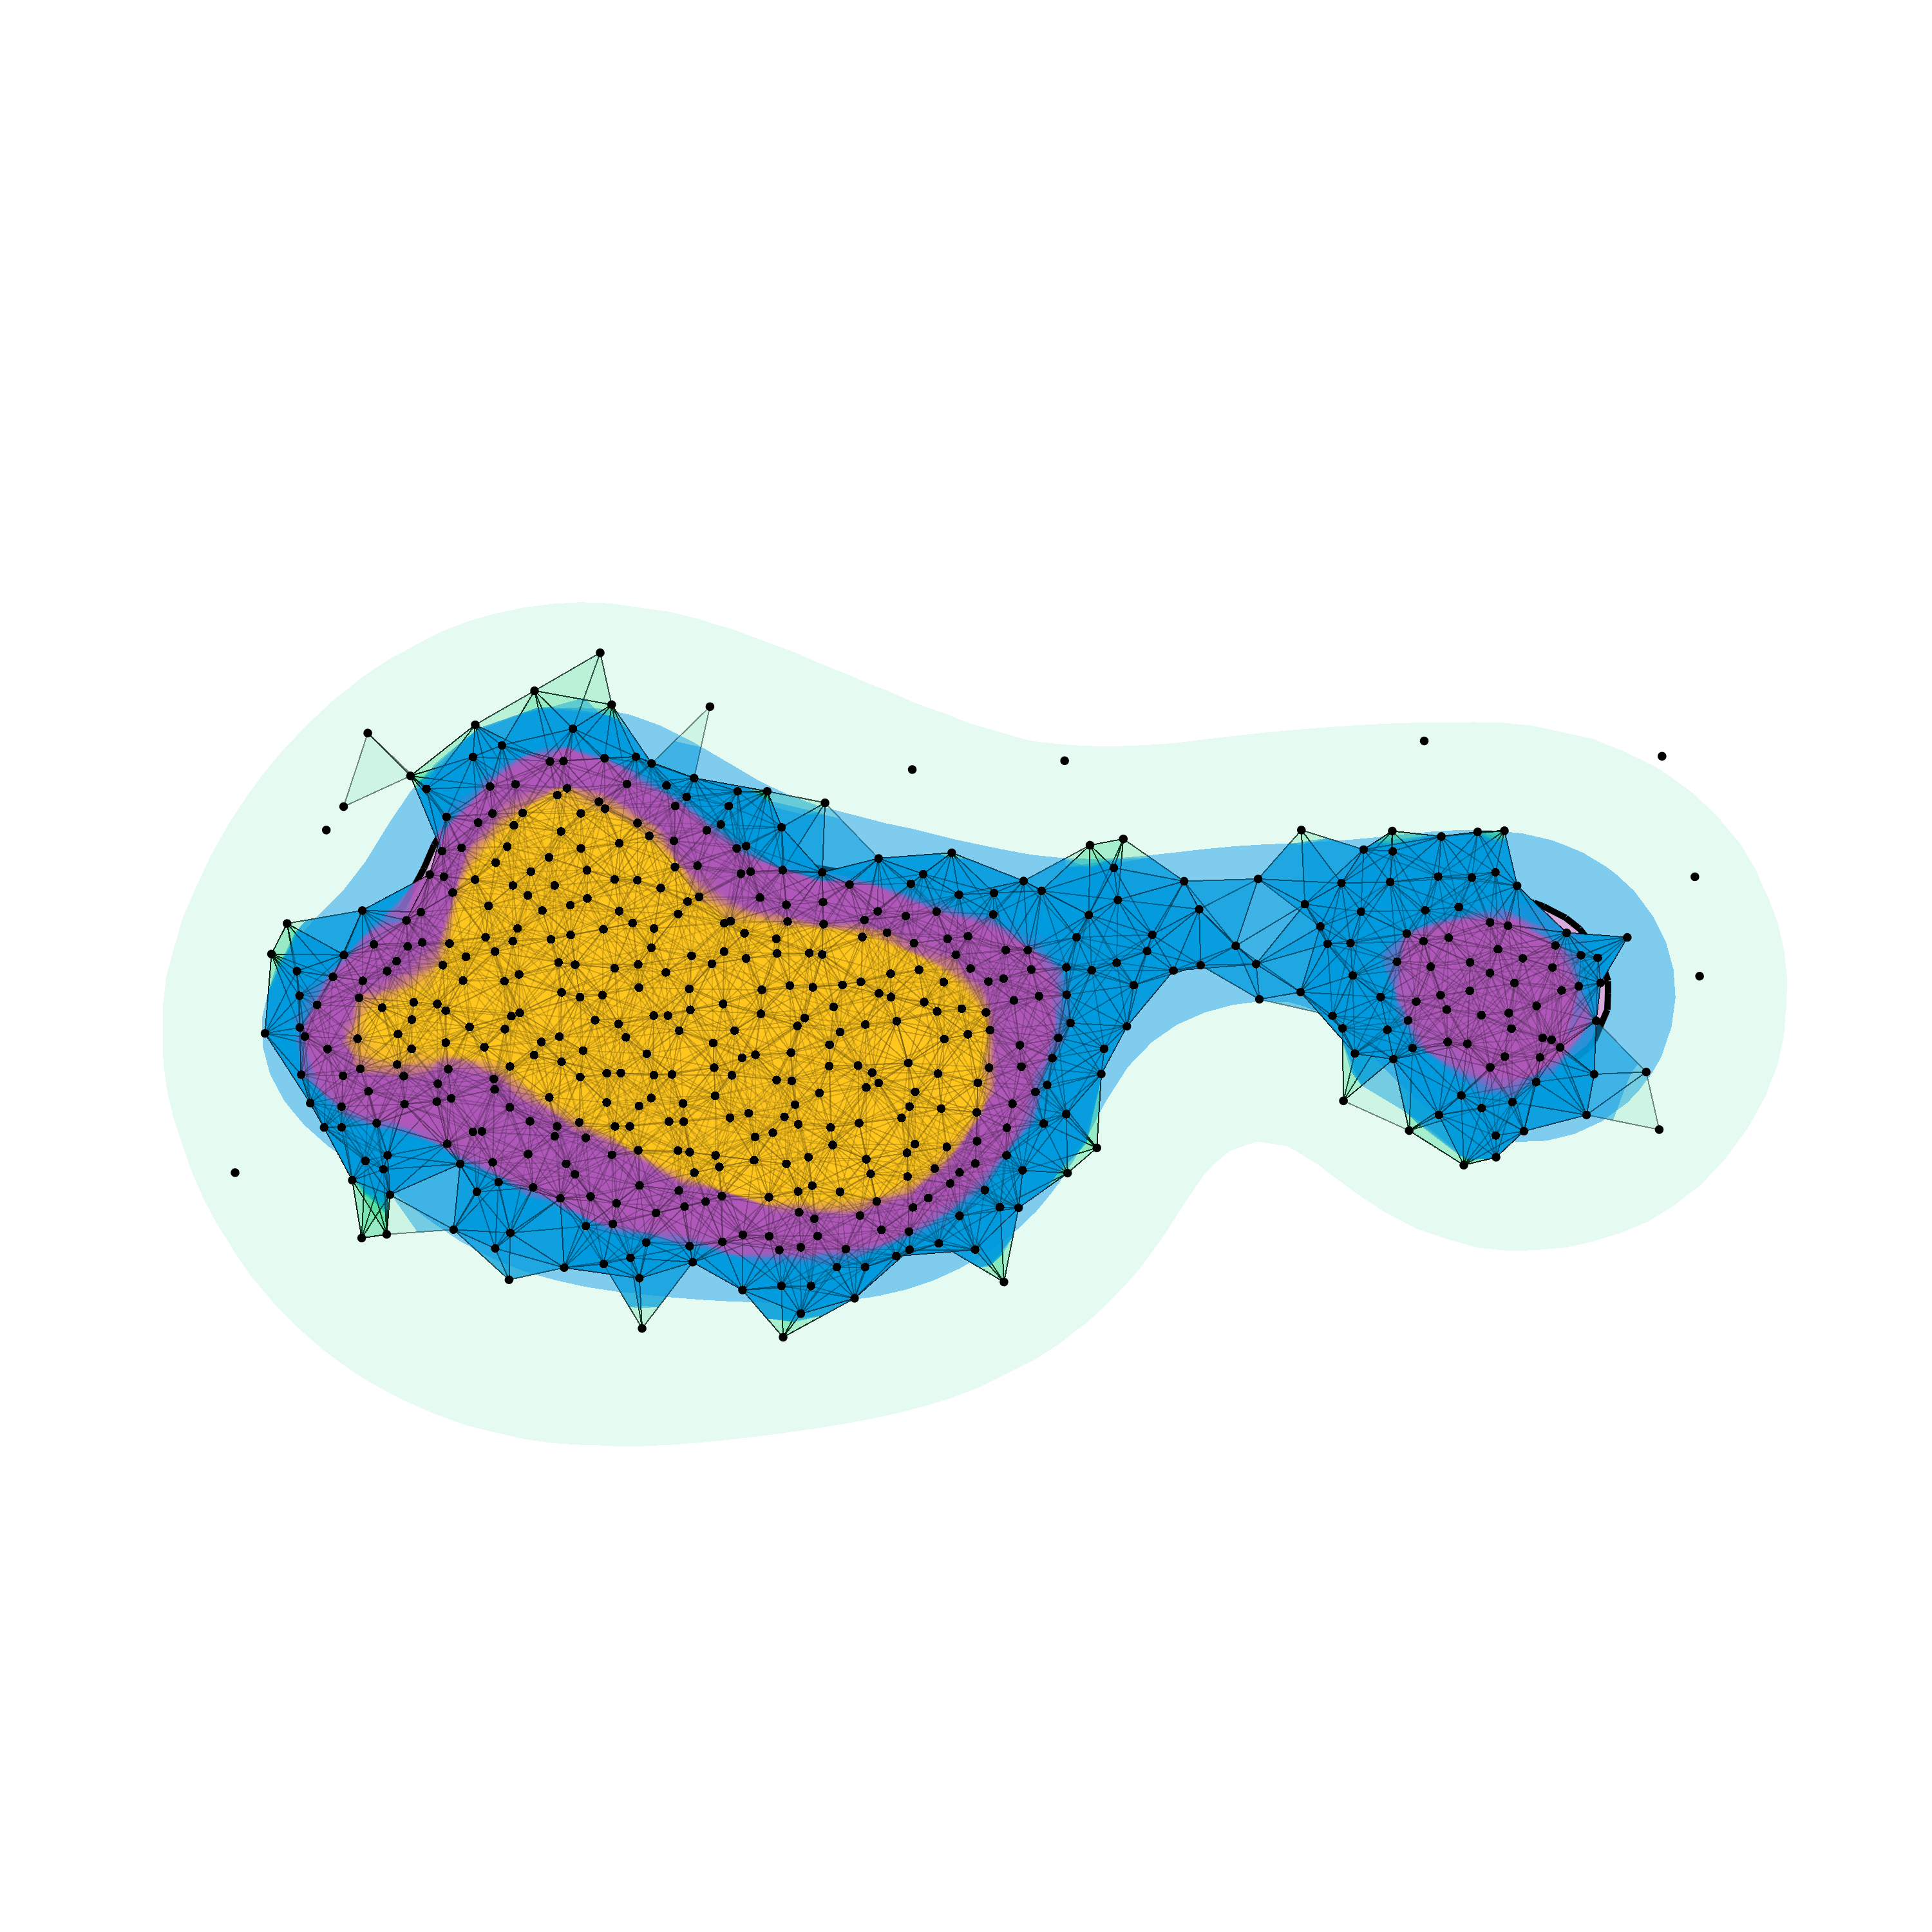
\includegraphics[trim=200 600 200 800, clip, width=0.5\textwidth]{figures/samples/scalar1}
  \end{textblock*}
\end{frame}
